\documentclass[17pt]{article}
\usepackage[top=1.4cm,bottom=1.4cm,left=1cm,right=1cm]{geometry}
%\usepackage{fontspec}
\usepackage[utf8]{inputenc}
\usepackage{hyperref}
\usepackage{enumitem}
\usepackage{changepage}
\usepackage[table]{xcolor}
\usepackage{graphicx}
\usepackage{fancyhdr}
\pagestyle{fancy}
\hypersetup{
	colorlinks=true,      
	urlcolor=magenta,
}

\title{\Huge{\textbf{Tiva Based Daughter Board for Firebird V \\ Hardware And Software Manual.}}}

\author{\textbf{ eRTS Lab IIT Bombay}}

\rhead{Manual for Tiva Based Daughter Board for Firebird V.}
\lfoot{eRTS Lab IIT Bombay}

\begin{document}
	\maketitle
	\newpage
	\section{\Huge{\textbf{Credits}}}
	\textbf{\\ \\ Version 1.0\\ \date{\today}}% Right allign
	\\
	\\
	\\
	\\
	{\large{\textbf{Documentation Author(Alphabetical Order):}
			\begin{enumerate}
			\item Ayush Gaurav, Intern eYSIP 2017
			\item Nagesh K,  Intern eYSIP 2017
	\end{enumerate}
	\textbf{Credits(Alphabetical Order):}
		\begin{enumerate}
			\item Prof Kavi Arya, CSE IIT Bombay
			\item Nex Robotics Pvt. Ltd.
			\item Piyush Manavar, Team e-Yantra
	\end{enumerate}}
	\newpage
	\section{\Huge{\textbf{Notice}}}
	{\large The contents of this manual are subject to change without notice. All efforts have been made to
	ensure the accuracy of contents in this manual. However, should any errors be detected, e-yantra welcomes your corrections. You can send us your queries / suggestions at
	\href{mailto:helpdesk@eyantra.org}{Contact Us}\\}
	\newpage
	\section{\Huge{\textbf{Index}}}%centre Allign This
	\begin{enumerate}
		\item 
	\end{enumerate}
	\newpage 
	\section{\Huge\textbf{Introduction}}
	\section{\Huge\textbf{Tiva Based Daughter Board}}
		\subsection{{\huge \textbf{Technical Specification}}}
		\subsection{}%start with the functionality
	\section{\Huge\textbf{Hardware Manual:}}
	\section{\Huge\textbf{Software Manual:}}
		\subsection{\huge \textbf{Code Composer Studio:}}
			{\large Code Composer Studio is an integrated development environment (IDE) that supports TI's Microcontroller and Embedded Processors portfolio. Code Composer Studio comprises a suite of tools used to develop and debug embedded applications. It includes an optimizing C/C++ compiler, source code editor, project build environment, debugger, profiler, and many other features. The intuitive IDE provides a single user interface taking you through each step of the application development flow. Familiar tools and interfaces allow users to get started faster than ever before. Code Composer Studio combines the advantages of the Eclipse software framework with advanced embedded debug capabilities from TI resulting in a compelling feature-rich development environment for embedded developers. This description is directly taken from the website of Texas Instruments and click to know more	\href{http://www.ti.com/tool/ccstudio}{about CC Studio}\\}}%Add an image of cc studio.
			\subsubsection{\Large\textbf{Download CC Studio:}}
			{\large At the time of writing this document Version 7 was the latest one. You can check for the latest at \href{http://processors.wiki.ti.com/index.php/Download_CCS}{Download CCS}.(do not download
				any beta versions).There will be two installer files.The web installer will require Internet access until it	completes. If the web installer version is unavailable or you can’t get it to work,
				download, unzip and run the offline version. The offline download will be much larger
				than the installed size of CCS since it includes all the possible supported hardware.}
			\subsubsection{\Large\textbf{Installing C C Studio:}}
				{After the installer has started follow the steps mentioned below:\\
				\begin{enumerate}
					\item Accept the Software License Agreement and click Next.\\
							{\centering
							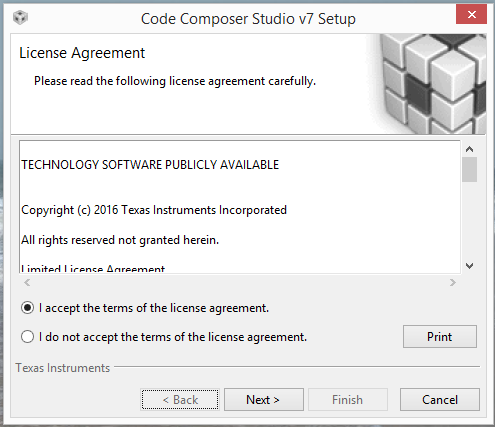
\includegraphics[width=6cm, height=6cm]{CCSInstall1}}
					\item Select the destination folder and click next.\\
							{\centering
							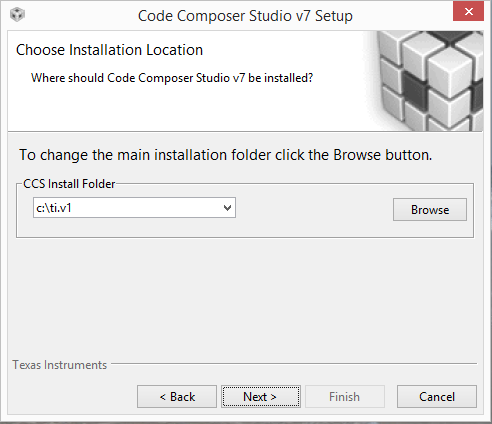
\includegraphics[width=6cm, height=6cm]{CCSInstall2}}
					\item Select the processors that your CCS installation will support. You
						must select "TM4C12X Arm Cortex M4". You can select other architectures, but the installation time and size will increase.\\{\centering
							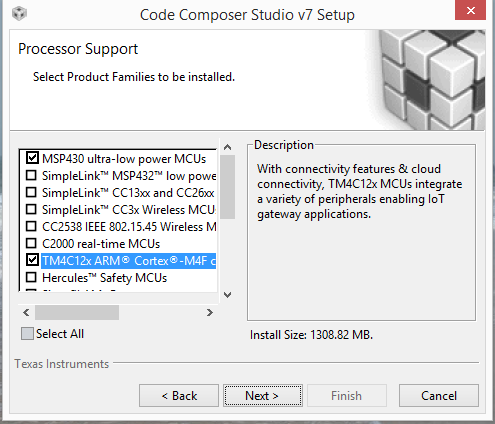
\includegraphics[width=6cm, height=6cm]{CCSInstall3}}
					\item Select debug probes and click finish \\
							{\centering
							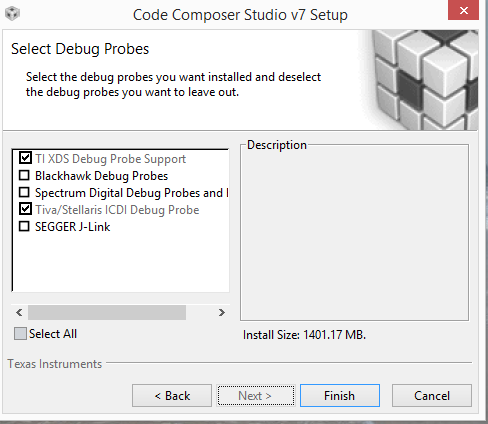
\includegraphics[width=6cm, height=6cm]{CCSInstall4}}
					\item The installer process	should take 15 - 30 minutes, depending on the speed of your connection. The offline
					installation should take 10 to 15 minutes. When the installation is complete, uncheck the
					“Launch Code Composer Studio v7” checkbox and then click Finish.There are several additional tools that require installation during the CCS install process. Click “Yes” or “OK” to proceed when these appear. \\
				\end{enumerate}}
				
\end{document}